\newpage
%%%%%%%%%%%%%%%%%%%%%%%%%%%%%%%%%%%%%%%%%%%%%%%%%%%%%%%%%%%%%%%%%%%%%%%%%%%%%%%%
%%%%%%%%%%%%%%%%%%%%%%%%%%%%%%%%%%%%%%%%%%%%%%%%%%%%%%%%%%%%%%%%%%%%%%%%%%%%%%%%
\section{Percepção de frases musicais}
\label{sec:perceberfrases}
\index{Musicalidade!Frase musical}

As \hyperref[sec:Frase]{\textbf{frases musicais}} são medidas e classificadas pelo seu tipo de inicio e final,
como foi visto na Seção \ref{sec:Frase};
por outro lado, a forma e os critérios que são usados para agrupar frases musicais em estruturas maiores, 
é dizer a composição estruturada, 
é estudada nas seções \ref{sec:fraseio}, \ref{sec:estruturadamusica} e \ref{sec:compondoestruturadamente};
finalmente, um par de exemplos simples destas estruturas formadas por frases,
foi visto quando estudamos os \hyperref[sec:Periodo]{\textbf{períodos}} e 
as \hyperref[sec:sentence]{\textbf{sentenças}} nas Seções \ref{sec:Periodo} e \ref{sec:sentence}, 
respetivamente.

Nesta seção presentaremos critérios, para poder dividir uma música ou uma seção dela,
na suas frases musicais. 


\begin{tcbattention}
Uma coisa importante a ter em conta quando analisamos as frases de uma música,
é que estas tendem a ser percebidas de forma ambígua na introdução da música;
pelo fato que é nessa seção da peça, onde os compositores tem muita liberdade criativa,
e podem introduzir irregularidades no comprimento em relação ao corpo da peça. 
Por isso é recomendável iniciar nosso analises das frases no corpo da música. 
\end{tcbattention}

\subsection{Separando frases analiticamente}

Para poder identificar as frases musicais, 
nesta seção serão presentadas algumas dicas que usam informação extraída da teoria musical,
pelo que seu uso requer um mínimo de conhecimento teórico nesta área. 



\PRLsep{Frases de comprimento regular}

Na música popular, podemos achar peças com frases musicais com um comprimento regular,
é dizer, que  tem a mesma quantidade de compassos;
neste caso, uma forma de identificar e separar as frases musicais, 
é detetando uma frase na peça musical,
contar o número de compassos que esta contem, 
e usar esta medida para detetar e predizer as demais frases.


\begin{itemize}
\item Os comprimento de frase de 4 compassos  e 8 compassos 
são os mais comuns de serem vistos
\cite[pp. 624]{latham2008diccionario} \cite[pp. 335]{medteoria} \cite[pp. 34]{bennett1993elementos} %4
\cite[pp. 335]{medteoria} \cite[pp. 34]{bennett1993elementos}. %8
\item São incomuns frases de 3, 5, ou 7 compassos \cite[pp. 34]{bennett1993elementos}.
\end{itemize}
Assim, quando iniciemos a busca do comprimento de uma frase musical,
devemos ter em conta sempre o ditado: ``provavelmente 4 ou 8 compassos''.


\PRLsep{Frases de comprimento irregular}
Nas músicas dos subgêneros do samba, 
é mais comum achar peças com frases de comprimento irregular que as de comprimento regular;
porém, a estadística de comprimentos é a mesma,
sendo comum ver musicas compostas por frases de 4 e 8 compassos 
\cite[pp. 624]{latham2008diccionario} \cite[pp. 335]{medteoria} \cite[pp. 34]{bennett1993elementos} %4
\cite[pp. 335]{medteoria} \cite[pp. 34]{bennett1993elementos}; %8
também é possível ver com frequência, frases com 2 compassos de comprimento 
\cite[pp. 34]{bennett1993elementos},%2 
sendo usados para conectar frases mais longas.


\PRLsep{Contagem do número de compassos}

Quando contamos o comprimento de uma frase musical, 
devemos ter cuidado quando a frase inicia em tempo fraco,
pois se a frase musical é \hyperref[subsub:anacrustica]{\textbf{anacrústica}}\footnote{O 
tema da anacruse é estudado na Pag. \pageref{subsub:anacrustica}.},
então as notas presentes na anacruse não são contadas no comprimento da frase
\cite[pp. 148,150]{medteoria}, pelo que todo o compasso onde se acham as anacruses,
toma o nome de compasso zero e não é computado no comprimento da frase.
Na Figura \ref{fig:contagemtemposfrase} podemos ver uma serie de exemplos, 
de frases musicais, com formula de compassos 2/4, onde todas tem dois compassos de comprimento.
\begin{figure}[!h]
    \centering
    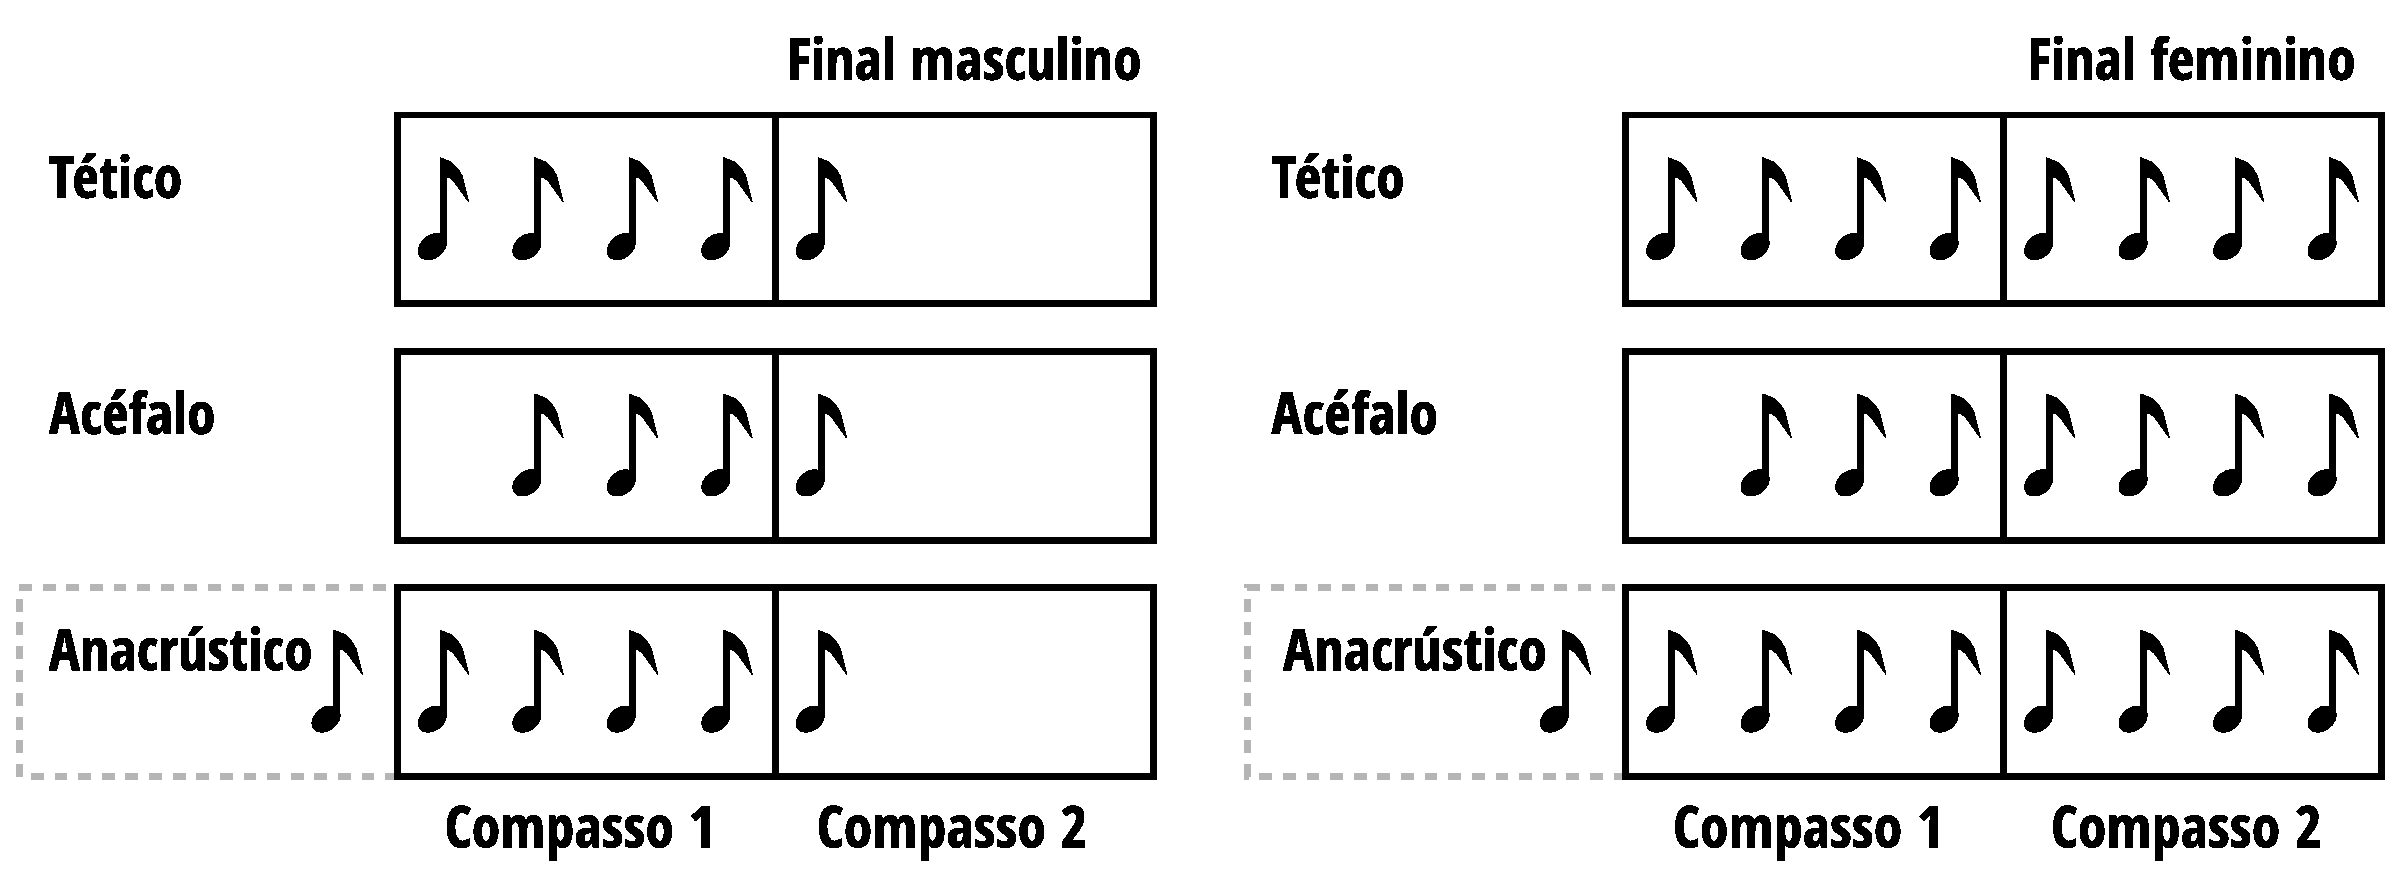
\includegraphics[width=\textwidth]{chapters/cap-musicalidade/contagemcompassosfrase.eps}
    \caption{Frases musicais com 2 compassos de comprimento.}
    \label{fig:contagemtemposfrase}
\end{figure}
É importante ressaltar, que não importa o número e a duração das notas ao final da frase,
o compasso final sempre é computado no comprimento;
mas, no caso das notas no inicio, isto não é assim,
pois o compasso que contem as anacruses não é computado.


\PRLsep{Detetando o inicio e o final de frase musical}


De forma geral, em músicas com textura \hyperref[subsec:monofonica]{\textbf{monofônica}} 
e \hyperref[subsec:homofonica]{\textbf{homofônica}} o acompanhamento percussivo ou harmônico,
tende a estar atrelado à melodia principal, 
pelo que identificar e seguir  as frases musicais pode ser mais simples no acompanhamento,
por ter uma caraterísticas regular e repetitiva.


%%%%%%%%%%%%%%%%%%%%%%%%%%%%%%%
\label{pos:detetandoiniciofrase}
Entre as dicas que podemos seguir para detetar o inicio de uma frase musical, encontramos que:
\begin{itemize}
\item Em musicas com textura monofônica e homofônica, podemos detetar o inicio da frase musical,
analisando a letra ou sua correspondente melodia principal;
se apos uma pausa, escutamos primeiro uma nota em tempo forte (\hyperref[subsub:Tetico]{\textbf{tética}}),
então temo achado o inicio da frase e começamos a contagem desde esse compasso;
por outro lado se escutamos primeiro uma nota em tempo fraco,
devemos analisar se o inicio é \hyperref[subsub:anacrustica]{\textbf{anacrústico}} ou 
\hyperref[subsub:Acefalo]{\textbf{acéfalo}}; 
se o inicio é anacrústico, 
as notas antes do primeiro tempo forte e seu compasso são descartadas da contagem;
no caso contrario, estamos frente um inicio acéfalo e o compasso sim é incluído na contagem. 
\item Existe geralmente, no primeiro tempo no primeiro compasso da frase, 
uma convergência de instrumentos de percussão, ou em geral do acompanhamento da melodia principal,
que provoca que este primeiro tempo forte seja percebido com uma maior \hyperref[sec:pos:Intensidade]{\textbf{intensidade}},
que os outros tempos fortes da frase;
pelo que esta tempo de maior intensidade pode servir como inicio da contagem.
\item Na música \hyperref[subsec:homofonica]{\textbf{homofônica}} as harmonias de acompanhamento estão geralmente submetidas
à frase da melodia principal; assim, pela regularidade deste acompanhamento harmônico,
pode ser mais simples procurar o inicio da frase na harmonia.
\end{itemize}~

%%%%%%%%%%%%%%%%%%%%%%%%%%%%%%%
\label{pos:detetandofinalfrase}
Entre as dicas que podemos seguir para detetar o final de uma frase musical, encontramos que:
\begin{itemize}
\item Geralmente entre o final de uma frase e o inicio de outra, 
existe um tempo de espera maior que o visto nas notas regulares da frase.
\item Podemos detetar o final de uma frase pois, 
ao ser interpretada como se fosse uma frase falada, 
percebemos que uma ideia tem sido completada.
\item Podemos aprender a reconhecer os tipos de \hyperref[sec:Cadencia]{\textbf{Cadência}},
vistas na Seção \ref{sec:Cadencia}.
\item Podemos prestar atenção ao \hyperref[ref:PontoCulminanteSuperior]{\textbf{ponto culminante superior}},
na frase musical, dado que indica que o final está próximo (ver Pag. \pageref{ref:PontoCulminanteSuperior}).
\item Podemos detetar o final da frase musical porque percebemos o inicio da seguinte.
\end{itemize}


\begin{example}[Músicas com frases de 4 compassos de comprimento:] ~
\label{ex:frasesde4compassos}
\begin{itemize}
\item ``Piston de gafieira'' de Billy Blanco.
\item ``Suingue de samba'' interpretado por Rogê.
\item ``Disritmia'' interpretado por Martinho da Vila.
\item ``Historia do samba'' interpretado por Joyce. % contando corporalmente é fácil de perceber.
\item ``impaciência'' interpretado por Luciana Mello.
%%%% quase regulares
\item ``Enfeitiçado'' interpretado por Aline Cardoso. 
Só tem uma frase de 3 compassos aproximadamente no meio da música.
\end{itemize}
\end{example}


\begin{example}[Músicas com frases de 8 compassos de comprimento:] ~
\begin{itemize}
\item ``Altar particular'' interpretado por Maria Gadú. 
\item ``A cada dia que passa'' interpretado por Emílio Santiago.
\end{itemize}
\end{example}

\subsection{Separando frases intuitivamente}

Quando a música inclui letra é mas fácil distinguir, intuitivamente, 
onde inicia e finaliza uma frase;
pois nosso cérebro está treinado para perceber e processar a fala e sua estrutura;
reconhecendo, automaticamente,
onde existem signos de pontuação como:
a virgula, o ponto e virgula, o ponto, o signo de admiração ou interrogação;
que descreve finais de frases e nos indicam o tipo ou proposito da frase que vem depois.

Porém este processamento, automático, não é exclusivo da fala num idioma em particular,
pois lembremos que quando escutamos a uma criança muito pequena tentando falar,
não conseguimos entender o significado dos seus balbucios, 
mas sim conseguimos perceber as frases, 
e identificar frases exclamativas e interrogativas,
frases afirmativas e suspensivas;
tudo isto sem precisar do conteúdo das palavras.

Assim, com um pouco de esforço e imaginação,
podemos assumir que os sons de um instrumento musical, 
são como os balbucios de crianças, e tentar extrair intuitivamente das melodias,
as frases musicais. 
 
~

\begin{example}[O discurso de ``la'']
\label{ex:discrusodela}
Usando unicamente a silaba ``la'', crie um discurso; por exemplo:
\begin{citando}%%
Lálala la lalá lá!\\
la lalá la lálala ...\\
la lalalá lála?\\
la lalá la lalalá.\\
\end{citando}%%
Logo proceda a ler acentuando, pausando e
executando signos de interrogação e admiração.

Perceba que o conteúdo das palavras não existe, 
porém pela expressividade na leitura,
é possível extrair dos sonidos produzidos,
onde existem acentos, pausas, e signos de admiração ou interrogação.
\end{example}

\begin{example}
Na música, ``Brasileirinho''  de Valdir Azevedo, 
ao extrair as frases musicais, 
acontecerá o mesmo que com o discurso de ``la'' visto no Exemplo \ref{ex:discrusodela};
observaremos que:
\begin{itemize}
\item Teremos uma noção dos acentos na melodia, e poderemos intuir fazendo um levantamento estatístico,
em que tempo está localizado o tempo forte; o analises terá que ser probabilístico,
pois existe na música, a acentuação de tempos fracos (\hyperref[sec:contratempo]{\textbf{contratempos}}); 
pelo que se alguns tempos não cumprem com nossa predição podemos catalogar eles como contratempos.
\item Podemos perceber as pausas, e deduzir que existe um final de \hyperref[sec:Frase]{\textbf{frase}} musical;
e intuir o uso de uma \hyperref[fig:Cesura]{\textbf{cesura}}.
\item Também podemos perceber diferentes formas de finalizar uma frase, 
que na linguagem falada associaríamos com o uso ou não de signos de admiração e exclamação;
no âmbito da música, temos algo similar com o uso das \hyperref[sec:Cadencia]{\textbf{cadencias}}.
Assim, cada tipo de cadência nos dará uma ideia diferente da função que cumpre a frase no discurso da peça musical,
e sim se precisa ou não uma frase de resposta.
\end{itemize}
\end{example}
